\subsection{Algoritmo evolutivo para la búsqueda de caos}

Se propuso emplear un método eurístico para buscar parámetros del sistema implementado de tal forma que se maximice la caoticidad de su salida.
Este algoritmo tiene la ventaja que realiza una búsqueda inteligente mediante el empleo de un algoritmo genético, lo que minimiza el tiempo de cómputo.

Un algoritmo evolutivo es un método de búsqueda dirigido basado en la probabilidad.
Un juego de entidades que representan posibles soluciones compite con otros, evolucionando en mejores soluciones \cite{Weise2009}.

Las entidades que representan posibles soluciones al problema son llamados \textit{cromosomas} y el grupo de cromosomas es llamados \textit{población inicial}.

Desde la población inicial, o los primeros padres, se genera un hijo mediante el cruce entre ellos.
Luego, ellos son mutados en forma aleatoria para crear la próxima generación.
Cada generación es comparada con la previa para descartar los ``peor adaptados" y así los coeficientes (cromosomas) mutan hacia los ``mejor adaptados".

Cuando se aplican estos algoritmos en funciones continuas, siempre convergen hacia el máximo local.
Sin embargo, si el espacio de coeficientes es fractal, existen áreas bien definidas en donde el la función objetivo es positiva, negativa, cero o no existente.
Este es el caso si la función a maximizar es el MLE y el espacio de exploración es el de parámetros.

\subsubsection{Resultados}

Para evaluar la viabilidad del método, se generó el siguiente algoritmo y se probó sobre el mapa logístico.

En la figura \ref{fig:diagramaflujo1} podemos ver el diagrama de flujo principal.
El bloque \textit{Evolution} fue descompuesto en otro sub-diagrama para simplificar la descripción.
Este segundo diagrama puede verse en la figura \ref{fig:diagramaflujo2}, esta surutina maneja la evolución de los parámetros.
%
\begin{figure}
	\centering
	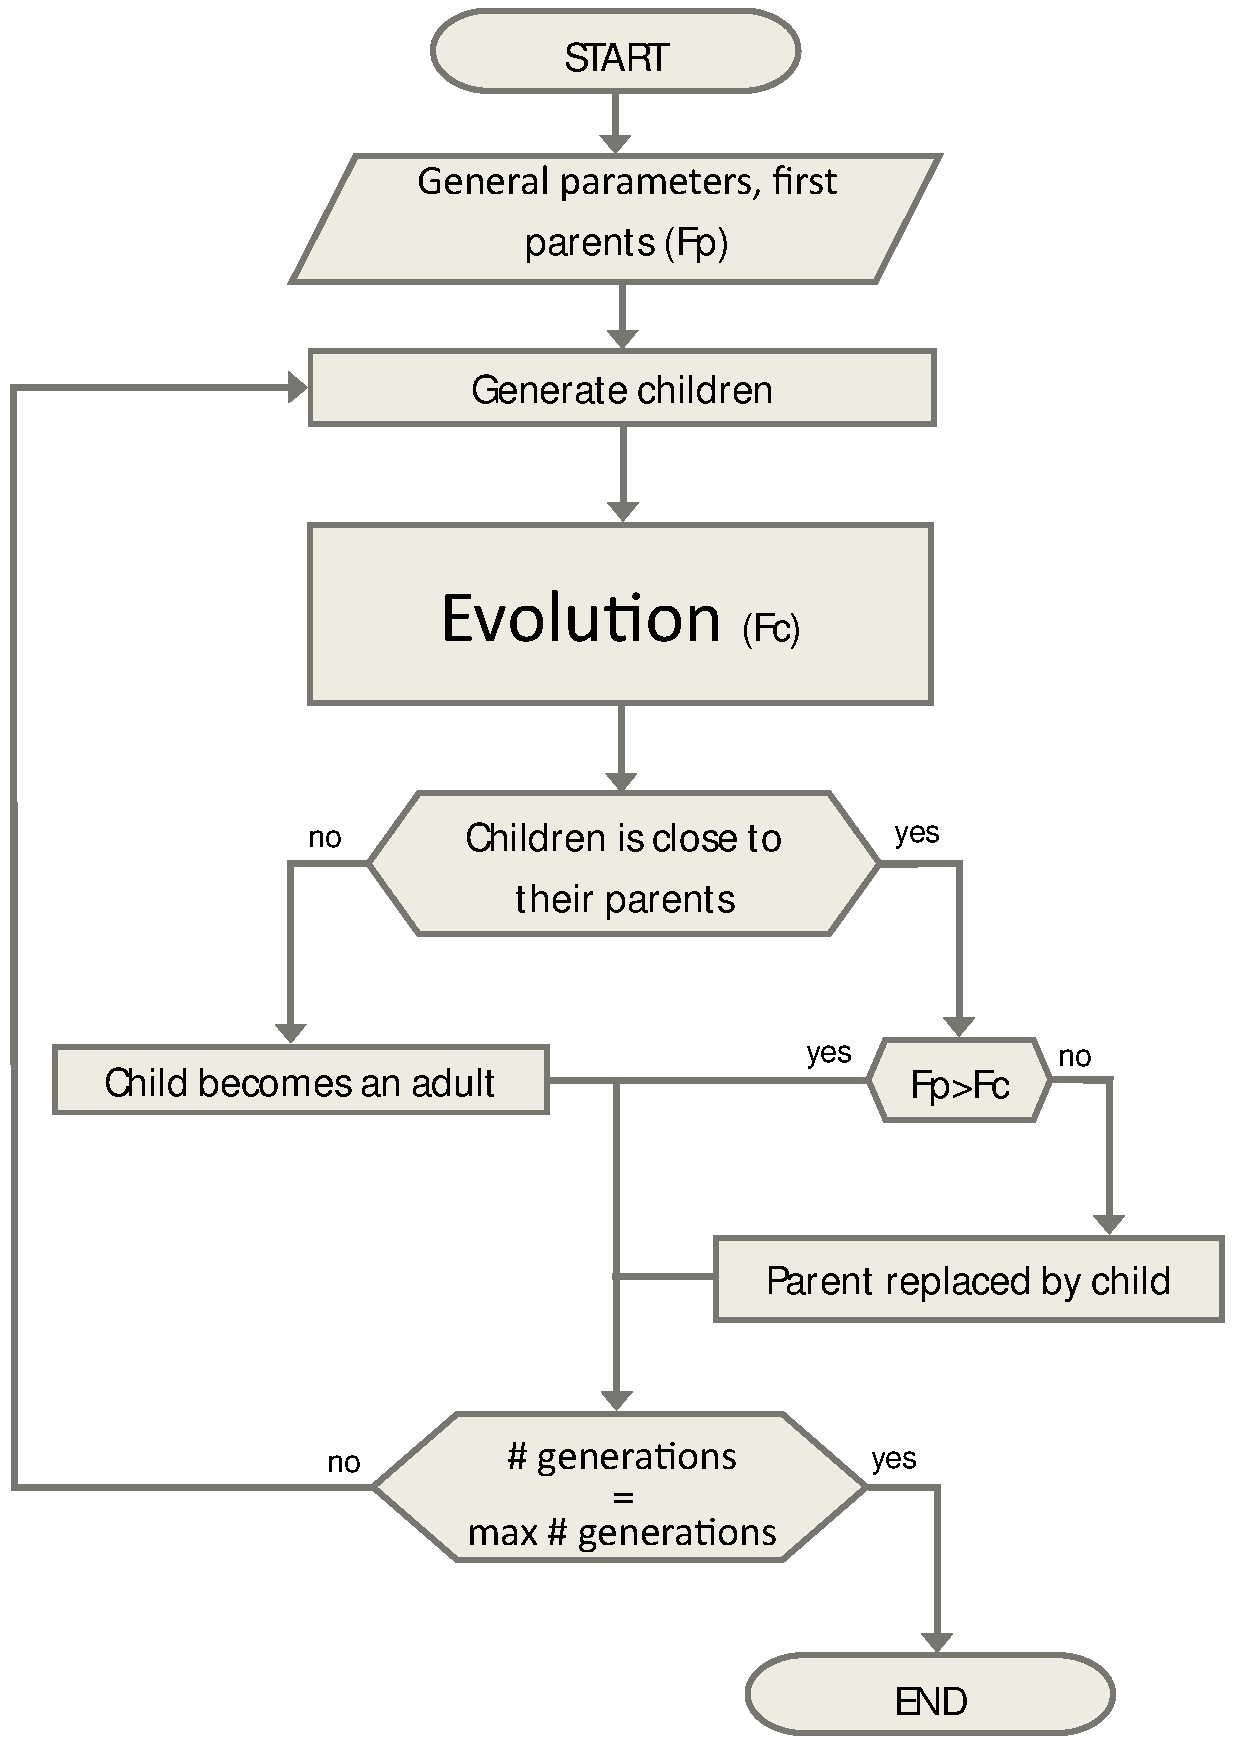
\includegraphics[width=0.9\columnwidth]{main_flowchart}\\
	\caption{Diagrama de flujo principal.}
	\label{fig:diagramaflujo1}
\end{figure}
%
\begin{figure}
	\centering
	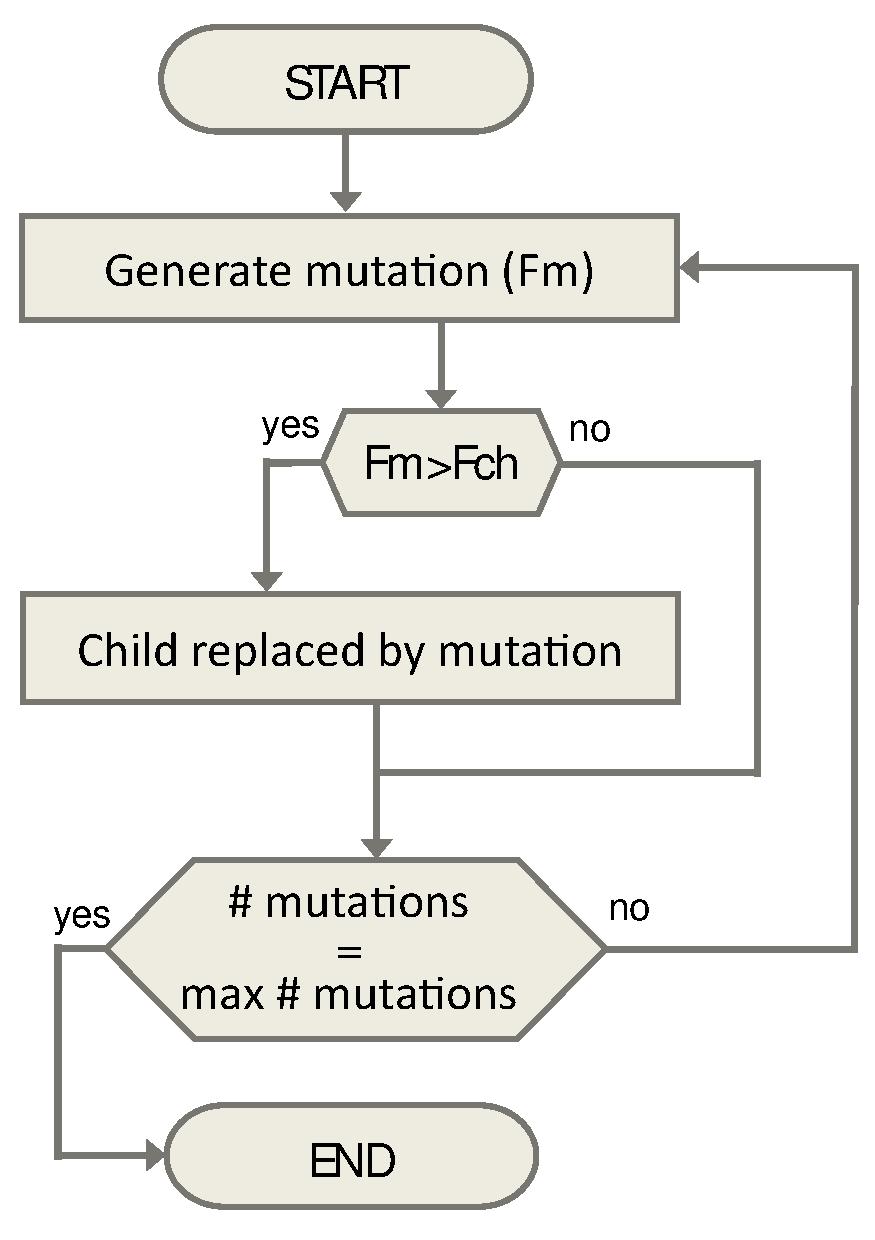
\includegraphics[width=0.56\columnwidth]{evolution_flowchart.pdf}\\
	\caption{Diagrama de flujo del bloque \textit{Evolution}.}\label{fig:diagramaflujo2}
\end{figure}

El algoritmo inicia con una inicialización general de parámetros como el número máximo de generaciones $max\_gen$, el número máximo de mutaciones $max\_mut$ y el número máximo de cambios en cada mutación $max\_stem$.
Luego se definen los primeros dos padres, ellos definirán los márgenes de búsqueda.
Además se calcula su \textit{fitness function} $Fp$.
A partir de este punto se itera la segunda generación, se elige en forma aleatoria un valor de parámetro $r$ con una distribución aleatoria entre los primeros dos padres, generando un nuevo hijo.
Luego este hijo entra en la subrutina \textit{Evolution} cuya salida es el valor de $r$ evolucionado y su correspondiente $Fc$.

Luego se evalúa si este hijo avolucionó muy cerca de sus padres o no.
Si la distancia entre ellos es más grande que el parámetro $max\_hop$, entonces este hijo es considerado como adulto, en caso contrario debe competir con su padre más cercano sobreviviendo el más apto.

Este proceso se repite hasta que se llega al máximo número de  generaciones $max\_gen$.
El grupo final de adultos es la solución al problema de buscar los máximos MLE locales.

La subrutina \textit{Evolution} de la figura \ref{fig:diagramaflujo2} es un algoritmo muy simple basado en mutaciones.
El primer paso es generar una mutación del hijo con una probabilidad uniformemente distribuida entre $\pm max\_step$, tambien se calcula su \textit{fitness function} $Fm$, que se compara con la del individuo original $Fc$.
Entonces sobrevive el mejor adaptado para dar lugar a la siguiente mutación.
Este procedimiento se repute hasta que se llega al máximo número de mutaciones $max\_mut$.

Como resultado podemos ver el $MLE$ del mapa logístico en función de su único parámetro $r$ en la figura \ref{fig:resultadoAlgorithm}.
La línea contínua muestra el $MLE$ en pasos continuos de $r$, mientras que los puntos destacados son el resultado del algoritmo propuesto.
%
\begin{figure}
	\centering
	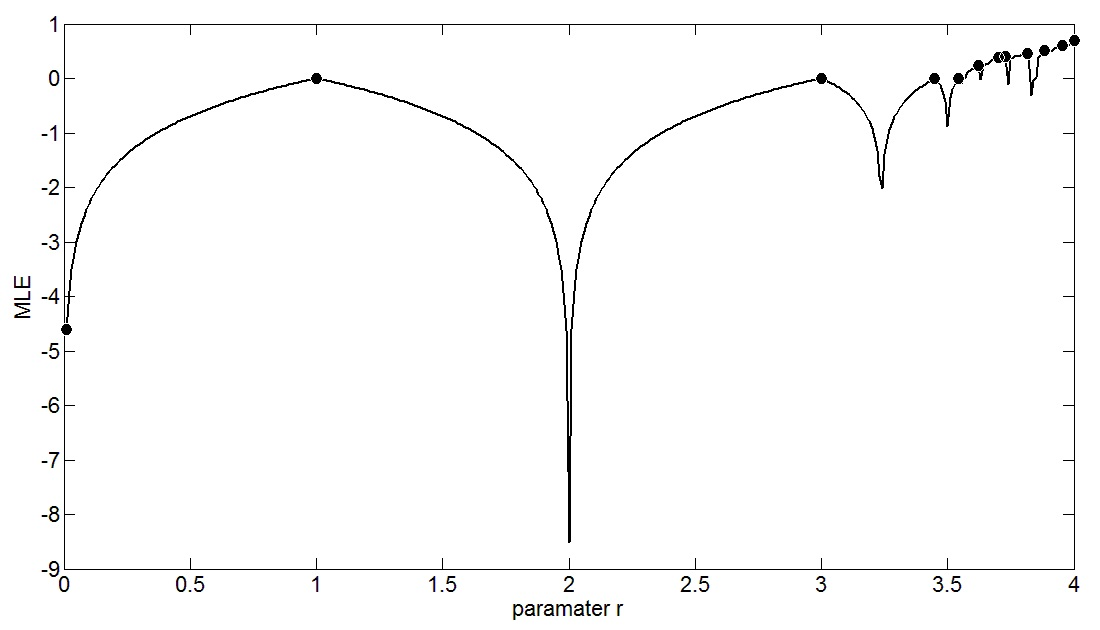
\includegraphics[width=1\columnwidth]{EvolutivoVSExaustivo.jpg}\\
	\caption{Resultados del algoritmo evolutivo para el mapa logístico, los puntos son los resultados del algoritmo.}\label{fig:resultadoAlgorithm}
\end{figure}

El bloque que calcula el $MLE$ fue sintetizado y verificado experimentalmente en un Altera CYCLONE III FPGA y los resultados de la compilación mostrados en la figura \ref{fig:compilacion}.
Los resultados del \textit{Timing Analysis} reportan que la máxima frecuancia es de $84.95MHz$.
El reporte de compilación muestra que la utilización de la lógica no excede el $20\%$, es decir un total de $20307$ de elementos lógicos, $54\%$ de los bits de memoria totales y $8\%$ de los multiplicadores embebidos.
%
\begin{figure}
	\centering
	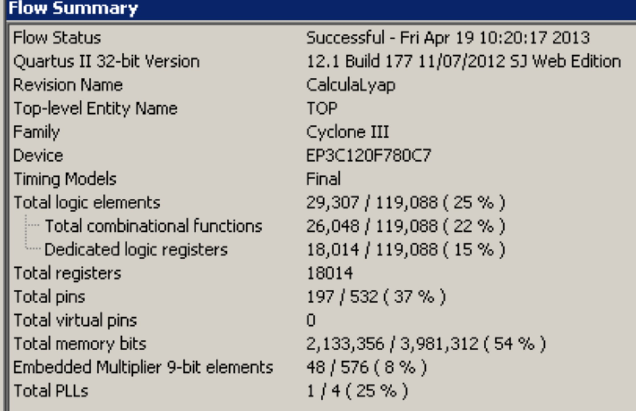
\includegraphics[width=1\columnwidth]{compilacion.pdf}\\
	\caption{Compilation report of the \textit{MLE} calculator.}\label{fig:compilacion}
\end{figure}

En la figura \ref{fig:st} se muestra la salida del Signal Tap.
La señal \textit{salida} es la suma de los $MLE$ luego de cada iteración.
La segunda señal llamada \textit{cuenta\_sal} corresponde a la sumatoria actual.
Finalmente, cada flanco descendente de la señal \textit{listoD1} indica que la salida es un dato válido.
La salida fué procesada con Matlab para obtener la curva mostrada en la figura\ref{fig:lyapu}.
El valor del MLE en la iteración $250000$ es $0.1415$, lo que es consistente con el MLE obtenido con Matlab.
%
\begin{figure*}
	\centering
	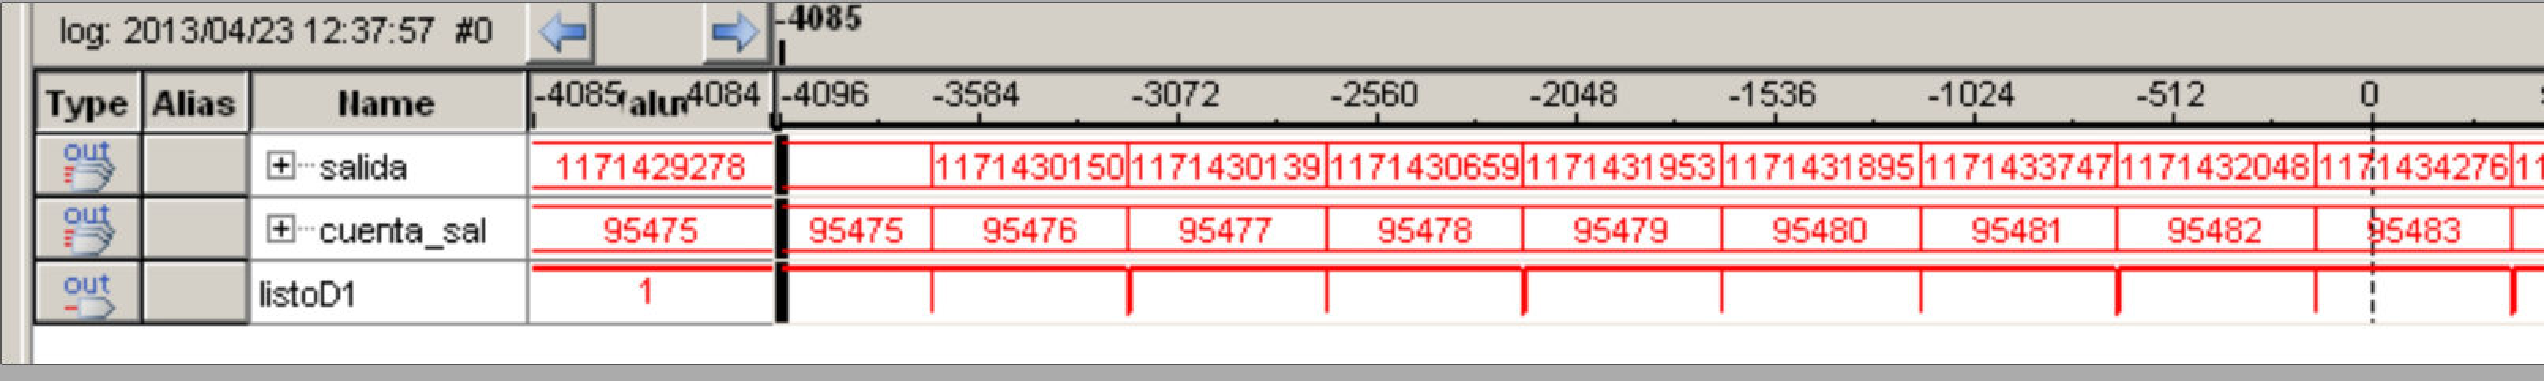
\includegraphics[width=1\columnwidth]{st.pdf}\\
	\caption{Salida del Signal Tap.}\label{fig:st}
\end{figure*}
%
\begin{figure}
	\centering
	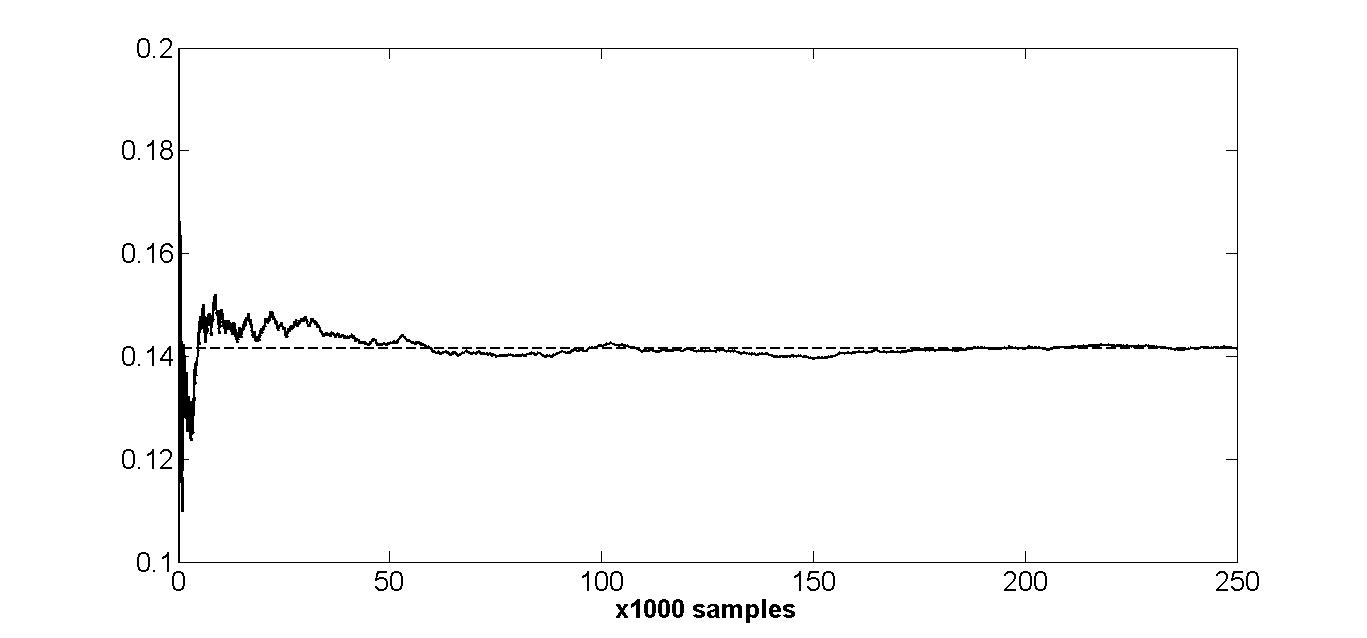
\includegraphics[width=1\columnwidth]{Lyap_MATLAB.jpg}\\
	\caption{Convergencia del algoritmo que calcula el MLE.}\label{fig:lyapu}
\end{figure}


\subsubsection{Estado actual del avance}

Actualmente estamos en etapa de desarrollo de la implementación en hardware de este algoritmo.
En este segundo caso, el sistema bajo prueba es la familia de mapas cuadráticos bidimensionales descriptos en la sección \ref{ssecQMaps}.

La población inicial es de $12$ coeficientes iniciales del mapa caótico empleado.
En la figura \ref{bloques} puede verse un diagrama en bloques general del sistema.
Este consiste en dos bloques principales conectados al sistema caótico bajo prueba a través de una interface wishbone.
Esto independiza el sistema del cuantificador y permite cambiar fácilmente el sistema bajo prueba.
%
\begin{figure}
	\centering
	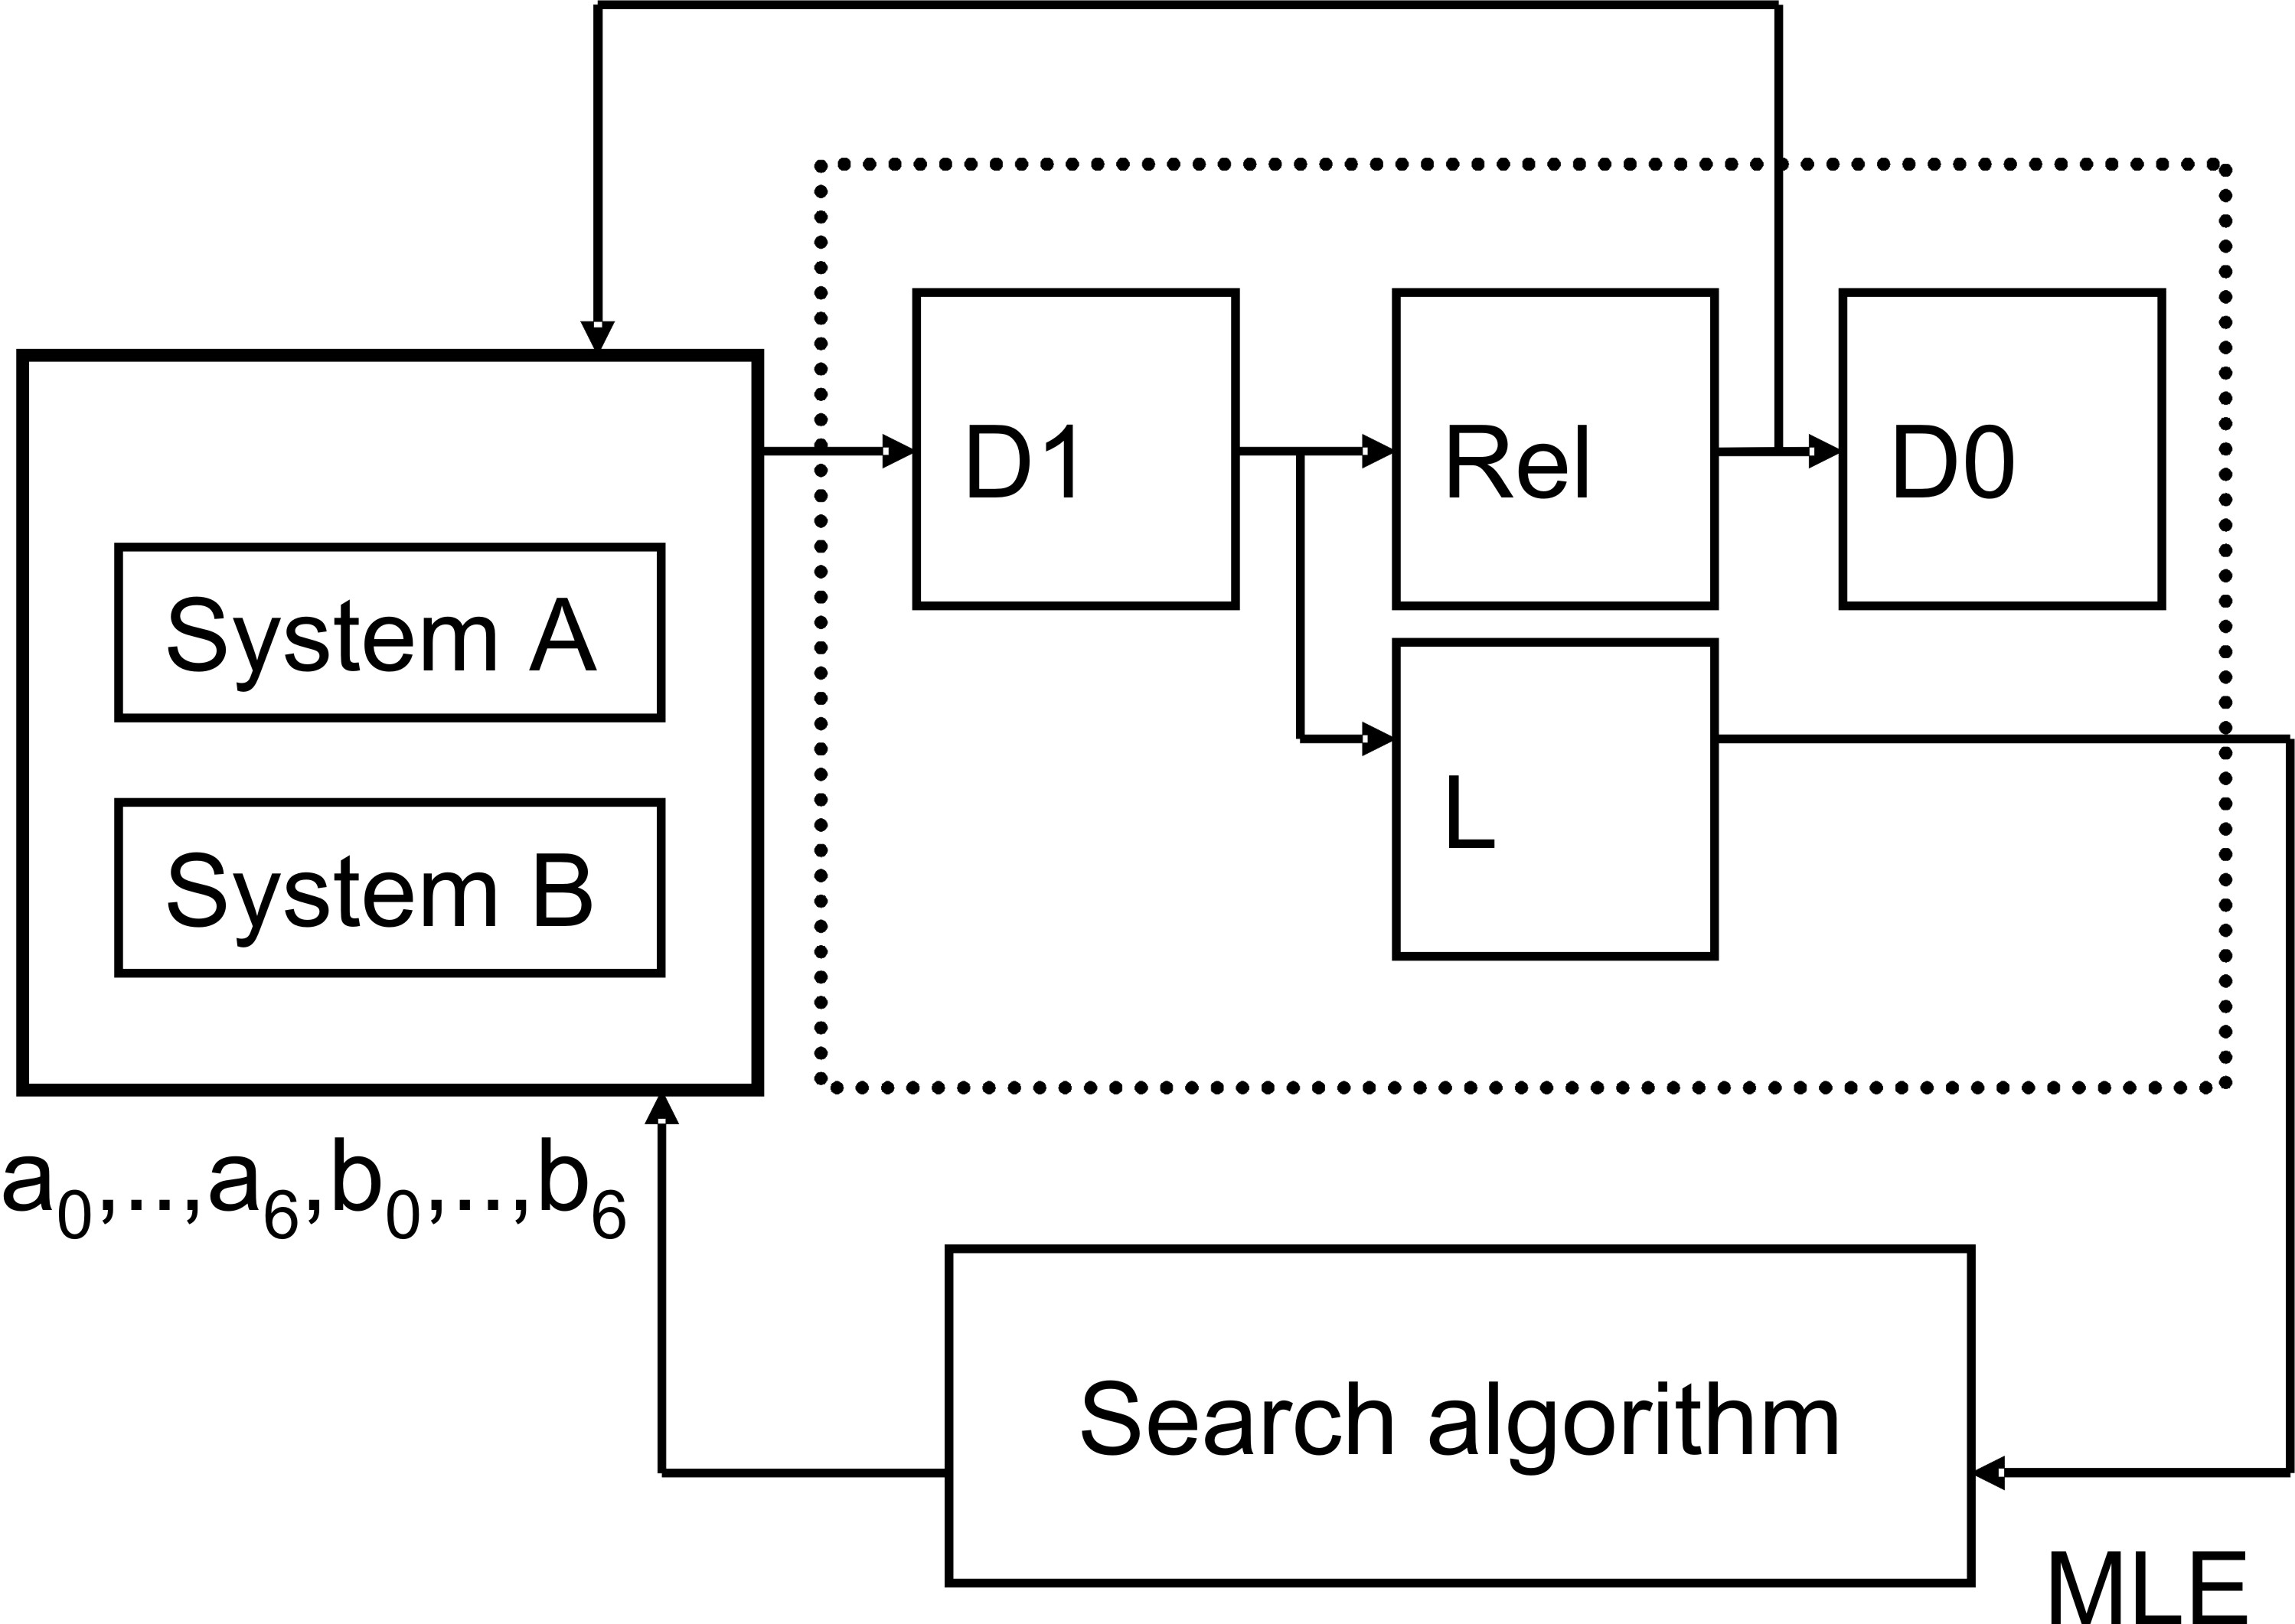
\includegraphics[width=0.85\columnwidth]{bloques.jpg}\\
	\caption{Diagrama en bloques del sistema implementado en FPGA.}\label{bloques}
\end{figure}

El sistema caótico es duplicado en dos bloques, $System A$ y $System B$.
Cada uno de ellos es inicializado con los puntos en el espacio de fases	($x_{a(i-1)}$,$y_{a(i-1)}$) y ($x_{br(i-1)}$,$y_{br(i-1)}$) respectivamente.
Cuando los sistemas caóticos terminan de calcular sus salidas, la señal digital \textit{habilita} se pone en cero y el bloque $D1$ es habilitado para calcular la distancia euclideana entre las salidas ($x_{a(i)}$,$y_{a(i)}$) y ($x_{br(i)}$,$y_{br(i)}$).

Luego se habilitan los bloques concurrentes $L$ y $Rel$.
Los puntos relocalizados que alimentan al bloque $System B$ son calculados por el bloque $Rel$.
Este bloque solo necesita los valores actuales de $d_1$ los valores previos de $d_0$, como se muestra en la ecuación \ref{eq:reubicacion}.
Cuando los puntos relocalizados $x_{br(i)}$ y $y_{br(i)}$ están disponibles, los bloques $System A$ y $System B$ se habilitan para obtener la siguiente iteración.
También se habilita el bloque $D_0$ para calcular el valor actual de $d_{0(i)}$, que se utilizará en la siguiente iteración.

Finalmente, el bloque $L$ realiza la división entre $d_0$ y $d_1$ para luego calcular el valor absoluto y el logaritmo de esta división.
El mapa es iterado $N=250000$ veces y el resultado de la sumatoria dividido por $N$ para asegurar la convergencia del método.

Cada bloque fue implementado utilizando lenguaje VHD e IP \textit{cores} provistos por \textit{Altera} (\textit{megafunctions}) cada vez que fue posible, debido a que estos \textit{cores} están optimizados para este dispositivo.
Las operaciones de punto flotante como las sumas, multiplicaciones, valores absolutos y logaritmos fueron calculadas con dichas \textit{megafunctions}.

La figura \ref{D1} muestra la implementación del bloque $D1$ en el entorno gráfico Quartus
Los puntos de salida y entrada $a$ y $b$, son tomados luego de que la señal \textit{habilita} se pone en cero.
Entonces, las señales son procesadas de acuerdo a la ecuación \ref{eq:D0D1} para calcular la distancia euclideana $d_1$.
%
\begin{figure*}
	\centering
	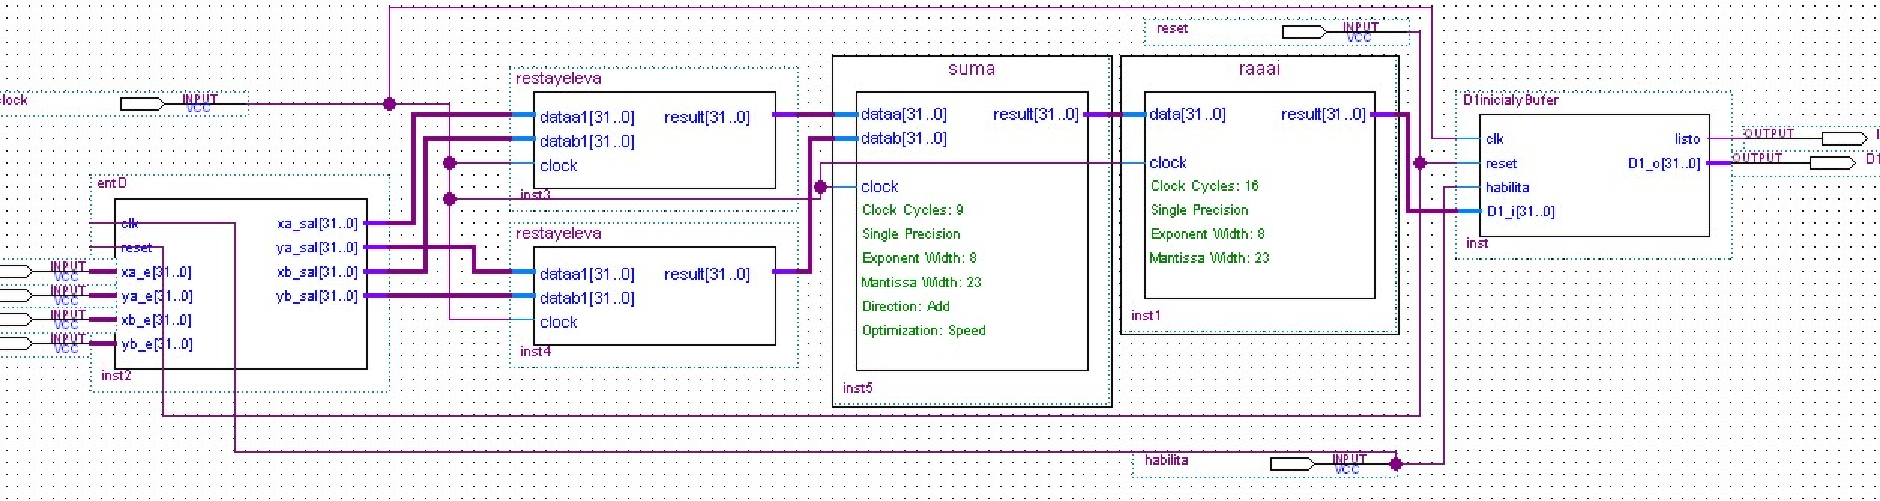
\includegraphics[width=1\columnwidth]{D1.pdf}\\
	\caption{Bloque $D_1$.}\label{D1}
\end{figure*}

La lógica del algoritmo genético fue implementada en lenguaje VHD.
Esta lógica junto con el registro de los $12$ coeficientes se muestran en la figura \ref{fig:evolutivecircuit}.
También se muesran los resultados de la compilación en la figura \ref{fig:alg_comp}.
Puede verse que esta implementación ocupa pocos recursos del dispositivo.
%
\begin{figure*}
	\centering
	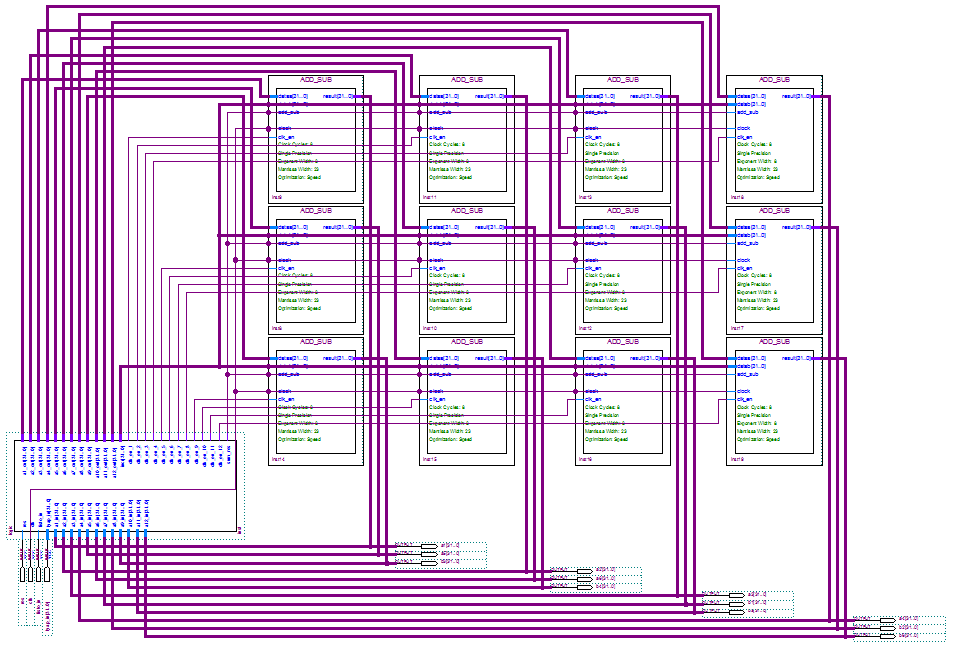
\includegraphics[width=1\columnwidth]{evolutive.png}\\
	\caption{Circuito del algoritmo evolutivo. Cada uno de los $12$ bloques ADD\_SUB guarda el valor de uno de los coeficientes $a_i$.}\label{fig:evolutivecircuit}
\end{figure*}
%
\begin{figure}
	\centering
	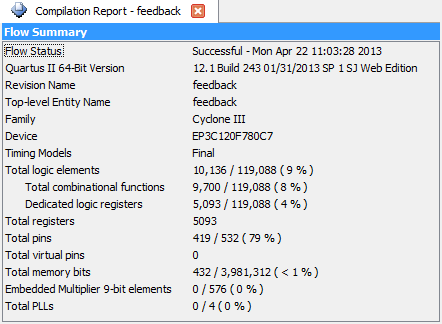
\includegraphics[width=1\columnwidth]{compilationreportalgoritmo.png}\\
	\caption{Compilation report del algoritmo evolutivo.}\label{fig:alg_comp}
\end{figure}